\documentclass[show notes]{beamer}
\usetheme{Rochester}

\usepackage{graphicx}
\usepackage{amsmath,amssymb}
\usepackage{ gensymb }

\title{Advanced Projects in Exoplanets}
\subtitle{The RM Effect}
\author{Dina Sofia Mortensen \& Jesper Dam Knudgaard}
\institute{Stellar Astrophysics Centre, Aarhus University}
\date{\today}

\begin{document}

\begin{frame}
\titlepage
\end{frame}

\section{The RM Effect}

\begin{frame}
\frametitle{Transiting Exoplanets}
	\begin{figure}
		\centering
		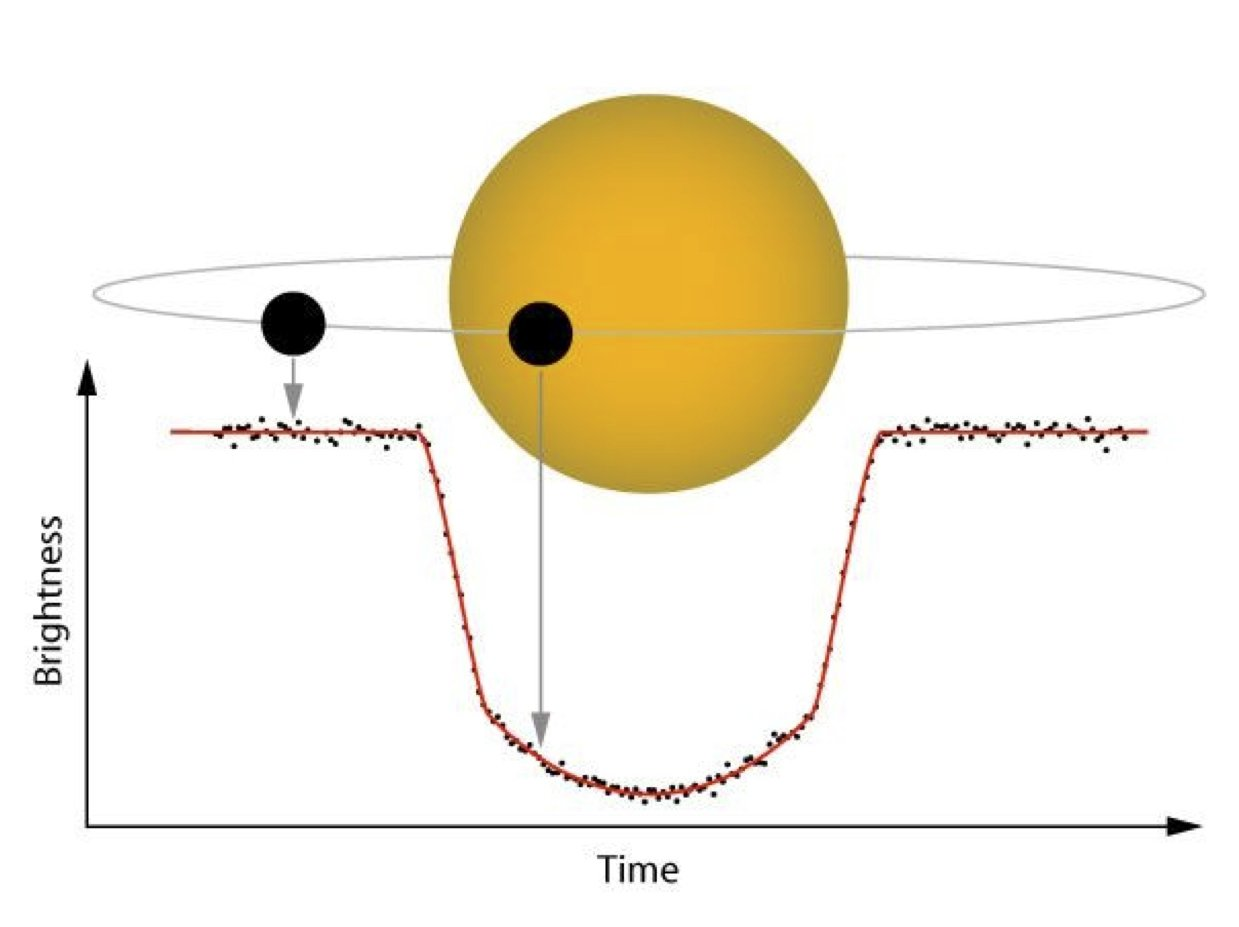
\includegraphics[width = 0.7\columnwidth]{Transit.jpg}
		\caption{\textit{Credit ESO}}
		\label{fig:transit} 
	\end{figure}
\end{frame}

\begin{frame}
\frametitle{Rossiter-McLaughlin Effect}
	\begin{figure}
		\centering
		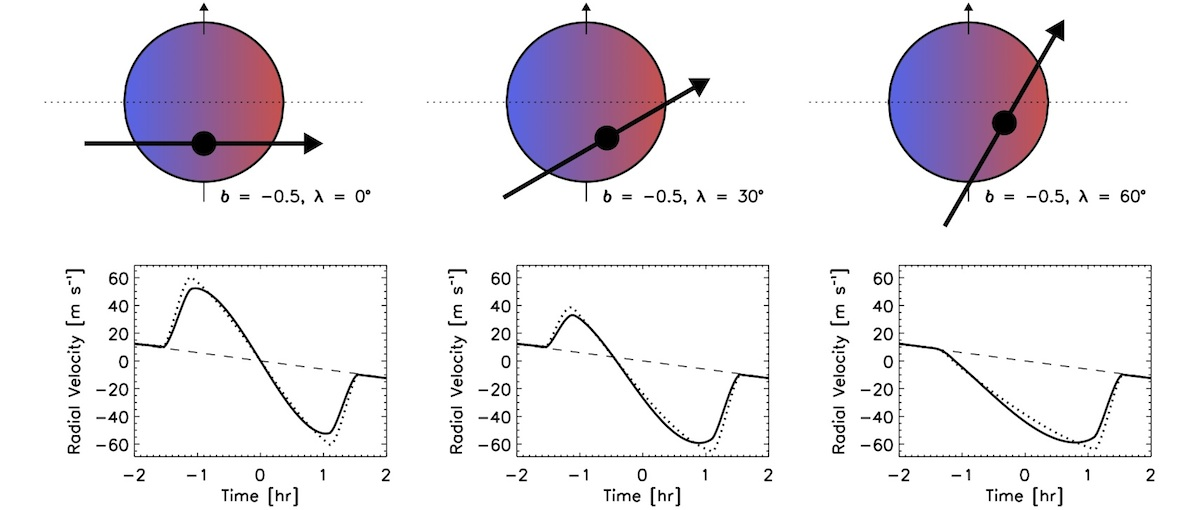
\includegraphics[width=\textwidth]{winnwhites.jpg}
		\caption{\url{https://wasp-planets.net/tag/rossiter-mclaughlin-effect/}}
		\label{fig:rm_effect}
	\end{figure}
\end{frame}

\note{Husk at nævne at det kun er projiceret obliquity vi kan måle, og det er fordi vi ikke ved hvordan stjernens rotationsakse er inklineret i forhold til os. }

\begin{frame}
\frametitle{}

\end{frame}

\section{Our Model}

\begin{frame}
\frametitle{Our Model - Linear}

\end{frame}


\begin{frame}
\frametitle{Keplers Equations}	
	
\end{frame}


\begin{frame}
\frametitle{Our Model - Physical version}

\end{frame}

\note{Vi laver her antagelsen at transit midpunkt sker til tiden t=0, og at $ \omega=90 $, så i tilfældet hvor vi har en eccentricitet, vil transitten ske ved periapsis.}

\begin{frame}
\frametitle{Our Model - Outputs}
	Her skal der stå noget om hvad det er vi ser på de forskellige figurer. Så det er her at vi viser vores animationer\\
	
	Vi skal snakke om hvordan vi bestemmer hvor vores centroid er, der er gauss-fittet, der ikke er godt, og så CM-metoden, som er meget bedre.
\end{frame}

\begin{frame}
\frametitle{Our Model - Outputs}

Så her tænker jeg at vi har selve RM-kurven. Så vi snakker noget om hvor fucked Gauss fittet er
\end{frame}

\begin{frame}
\frametitle{Data}
Lidt om systemet måske, og så en figur der viser en enkelt af CCF'erne
\end{frame}

\begin{frame}
\frametitle{Data - The Transit}
Figuren med de røde puntker, den hvor man ser RM-effekten for stjernen. Zoome ind på en af transitterne

\end{frame}

\begin{frame}
\frametitle{Data - The 'Planet Line'}

Den der figur hvor vi har en CCF, den gns. CCF, og en normeret CCF

\end{frame}

\begin{frame}
\frametitle{Data - The RM-effect}
	\begin{figure}
	\centering
%	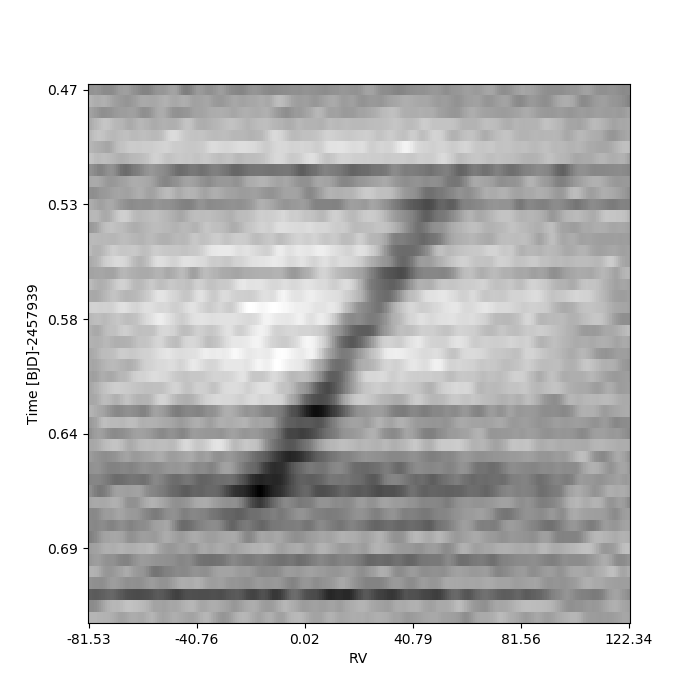
\includegraphics[width=\textwidth]{Colormap.png}
	\label{fig:colormap}
\end{figure}
\end{frame}


\begin{frame}
\frametitle{Data}
	\begin{figure}
	\centering
	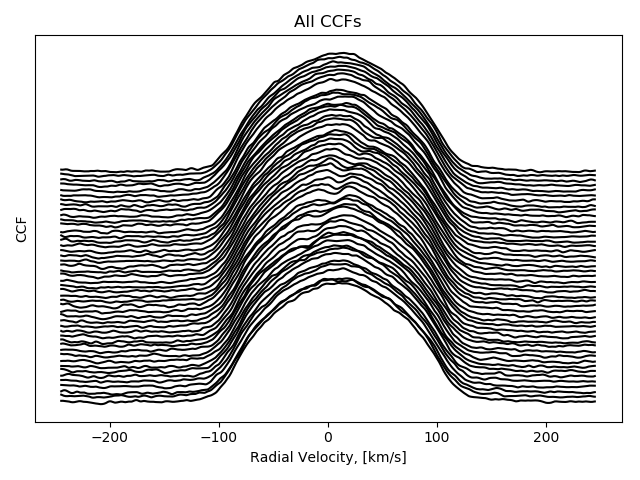
\includegraphics[width=0.8\textwidth]{All_CCFs.png}
	\label{fig:all_ccfs}
\end{figure}
\end{frame}

\begin{frame}
\frametitle{Data - RM curve}
	\begin{figure}
		\centering
		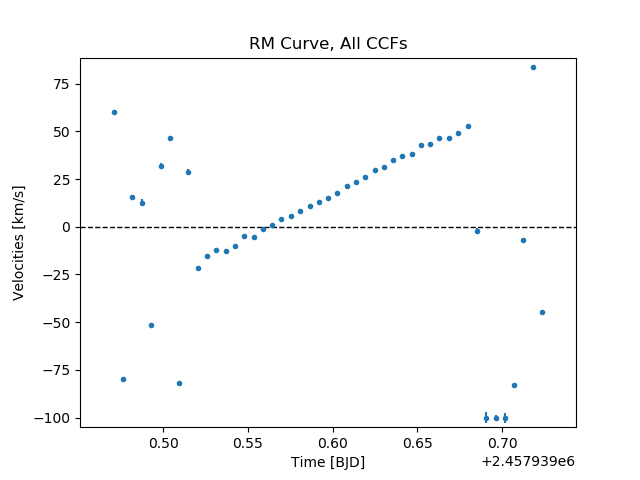
\includegraphics[width=0.8\textwidth]{RM_all_CCFs.png}
		\label{fig:RM_all_CCFs}
	\end{figure}
\end{frame}

\begin{frame}
\frametitle{Data - RM curve}
\begin{figure}
	\centering
	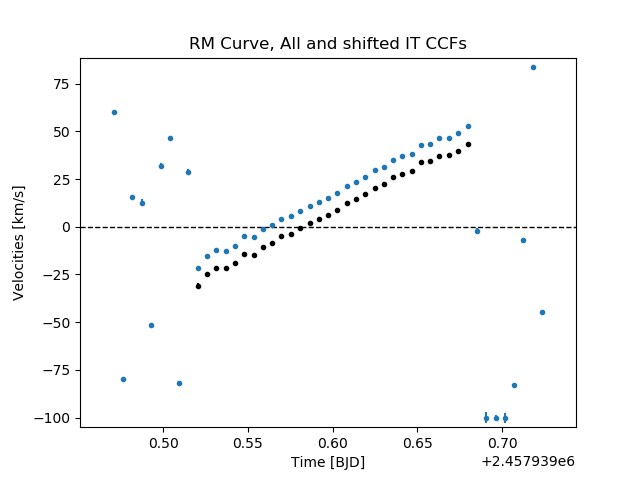
\includegraphics[width=0.8\textwidth]{RM_all_shift.png}
	\label{fig:RM_all_shift}
\end{figure}
\end{frame}

\begin{frame}
\frametitle{Data - RM curve}
\begin{figure}
	\centering
	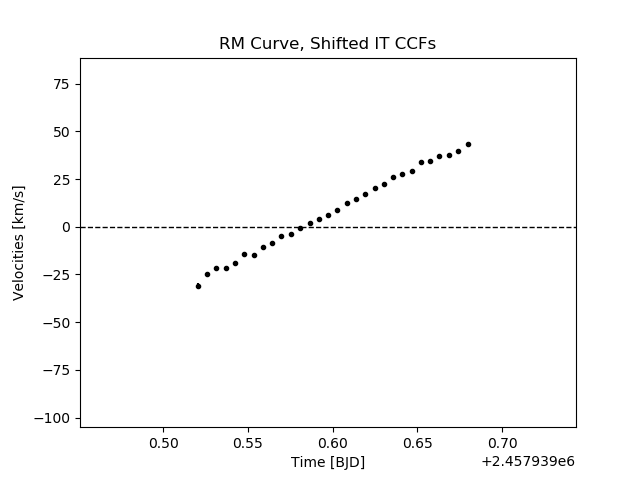
\includegraphics[width=0.8\textwidth]{RM_shift.png}
	\label{fig:RM_shift}
\end{figure}
\end{frame}

\begin{frame}
\frametitle{The Fit$ ^{\text{TM}} $}
\end{frame}


\end{document}
